%%%% DON'T CHANGE %%%%%%%%%
\documentclass[pmlr,twocolumn]{jmlr}% new name PMLR (Proceedings of Machine Learning Research)
%%%%%%%%%%%%%%%%%%%%%%%%%%%
   
% The following packages will be automatically loaded:
% amsmath, amssymb, natbib, graphicx, url, algorithm2e

%%% WARNING %%%%
%%% 1) Please, use the packages automatically loaded to manage references, write equations, and include figures and algorithms. The use of different packages could create problems in the generation of the camera-ready version. Please, follow the examples provided in this file.
%%% 2) References must be included in a .bib file.
%%% 3) Write your paper in a single .tex file.
%%%

%%%% SOFTWARE %%%%
%%% Many papers have associated code provided. If that is your case, include a link to the code in the paper as usual and provide a link to the code in the following comment too. We will use the link in the next comment when we generate the proceedings.
%%% Link to code: http://?? (only for camera ready)

 %\usepackage{rotating}% for sideways figures and tables
\usepackage{longtable}% for long tables

 % The booktabs package is used by this sample document
 % (it provides \toprule, \midrule and \bottomrule).
 % Remove the next line if you don't require it.
\usepackage{booktabs}
 % The siunitx package is used by this sample document
 % to align numbers in a column by their decimal point.
 % Remove the next line if you don't require it.
\usepackage[load-configurations=version-1]{siunitx} % newer version
 %\usepackage{siunitx}

 % The following command is just for this sample document:
\newcommand{\cs}[1]{\texttt{\char`\\#1}}

 % Define an unnumbered theorem just for this sample document:
\theorembodyfont{\upshape}
\theoremheaderfont{\scshape}
\theorempostheader{:}
\theoremsep{\newline}
\newtheorem*{note}{Note}

%%%% DON'T CHANGE %%%%%%%%%
\jmlrvolume{1}
\firstpageno{1}
\editors{List of editors' names}

\jmlryear{2022}
\jmlrworkshop{Machine Learning for Health (ML4H) 2022}

%\editor{Editor's name}
%%%%%%%%%%%%%%%%%%%%%%%%%%%

\title[ECG Scaling]{Exploring Best Practices for ECG Pre-Processing in Machine Learning}

%%%%%%%%%%%%%%%%%%%%%%%%%%%%%%%%%%%%%
% THE MANUSCRIPT, DATA AND CODE MUST BE ANONYMIZED DURING THE REVIEW PROCESS. 
% DON'T INCLUDE ANY INFORMATION ABOUT AUTHORS DURING THE REVIEW PROCESS.
% Information about authors (Full names, emails, affiliations) have to be provided only for the submission of the camera-ready version.  Only in that case, you can uncomment and use the next blocks.
%%%%%%%%%%%%%%%%%%%%%%%%%%%%%%%%%%%%%

 % Use \Name{Author Name} to specify the name.

 % Spaces are used to separate forenames from the surname so that
 % the surnames can be picked up for the page header and copyright footer.
 
 % If the surname contains spaces, enclose the surname
 % in braces, e.g. \Name{John {Smith Jones}} similarly
 % if the name has a "von" part, e.g \Name{Jane {de Winter}}.
 % If the first letter in the forenames is a diacritic
 % enclose the diacritic in braces, e.g. \Name{{\'E}louise Smith}

 % *** Make sure there's no spurious space before \nametag ***


  %Three or more authors with the same address:
\author{\Name{Amir Salimi} \Email{{asalimi@ualberta.ca}\\
\Name{Abram Hindle} \Email{abram.hindle@ualberta.ca}\\
\Name{Osmar Zaiane} \Email{zaiane@ualberta.ca}\\
\Name{others} \Email{CVC@ualberta.ca}\\
\addr University of Alberta}}



% added packages
\usepackage{xcolor} %just for notes
\begin{document}

\maketitle

\begin{abstract}
Are there any best practices for pre-processing of Electrocardiogram (ECG) signals for automatic diagnosis of heart disease? 
State of the art machine learning algorithms have achieved remarkable results in classification of heart disease using ECG data, yet there appears to be no consensus on how ECGs should be pre-processed.  Is this lack of consensus due to different diseases and model architectures requiring different pre-processing steps for optimal performance? Is it possible that state-of-the-art deep-learning models have rendered such pre-processing methods unnecessary? In this work we apply down-sampling, normalization, and filtering functions to 3 different multi-label ECG datasets and measure their effects on 3 different SOTA time-series classifiers. We find that sampling rates as low as 50Hz can yield comparable if not better results than the commonly used 500Hz sampling rate. This is significant as smaller sampling rates will result in smaller models, which in turn require less time and resources to train. (findings of normalization and filtering are pending)

\end{abstract}
\begin{keywords}
electrocardiogram, machine learning, signal processing
\end{keywords}


\section{Introduction}
% ecgs are used to diagnose heart conditions
% pre-processing functions can affect model accuracy and training complexity
% We wrote a project where we can test out pre-processing functions
% we ran an experiment on downsampling of ECGs, is the typical 500hz necessary?
\label{sec:intro}
In this work, we focus on data pre-processing decisions faced by researchers in the field of automatic classification of cardiovascular conditions using Electrocardiograms. The ever-growing number of tools and approaches available for machine learning often requires a number of a priori guesses to be made by those who process data and train models for machine learning tasks.
An Electrocardiogram (ECG) is a recording of the electrical activity of the cardiovascular system. ECGs are routinely utilized by clinicians for diagnoses of cardiovascular abnormalities. In recent years, machine learning models have achieved remarkable results in automatic diagnosis of some heart conditions when trained with enough labeled ECG data~\cite{reyna2021will,reyna4issues}. However, training such models requires a large amount of data~\cite{reyna2021will,reyna4issues,natarajan2020wide,ribeiro2020automatic}, where decisions regarding how the data is pre-processed (e.g., filtering, scaling, augmentation) can be critical for both the model's performance as well as the amount of time and hardware required. 


In order to automatically classify cardiovascular conditions using ECG data, we are faced with many choices for the pre-processing functions, due to the variety of implementations in previous works. Pre-processing functions are transformation functions applied to signals such as ECGs in order to reduce noise and simplify the learning task. Previous works utilize a diverse range of pre-processing functions, datasets, and architectures, often with great results~\cite{hong2022practical}. We believe that in order to make claims about the viability of ECG pre-processing methods (that is, whether they result in better outcomes, and their effect on time and hardware requirements) it is best to consider multiple datasets, architectures, and heart conditions.  


In this work we aim to simplify this decision space for other researchers by using our code to test the effect of \textit{down-sampling}, \textit{band-passing}, and \textit{normalizing} on the outcome of 3 different multi-label SOTA classifiers for time-series when trained on 3 different ECG datasets. We show that down-sampling from the standard recording rate of 500Hz can significantly reduce training times and hardware requirements, without being detrimental to model performance. In Section~\ref{sec:experiment} we discuss the experiment setup and results.  {\color{red} will also include quick summary of bandpassing and normalizing results}\\



\begin{table*}[tbp]
\label{tab:top5}
{\caption{Top 5 teams in Physionet2020 and pre-processing functions used.}}%
    
    { 
    \resizebox{1 \textwidth}{!}{
    \begin{tabular}{|c|c|c|c|c|}
    \hline
    Rank & Group                                          & Scaling                   & Normalize            & BandPass                  \\ \hline
    1    & Wide and Deep Transformer~\cite{natarajan2020wide}                   &                           & \checkmark & \checkmark \\ \hline
    2    & Adaptive ResNet~\cite{zhao2020adaptive}                  & \checkmark & \checkmark & \\ \hline
    3    & SE-ResNet~\cite{zhu2020classification}        &                           &                           &                           \\ \hline
    4    & Scatter Transform and DNNs ~\cite{oppelt2020combining}             &                           & \checkmark &                           \\ \hline
    5    & Adversarial Domain Generalization~\cite{hasani2020classification}&                           &                           & \checkmark \\ \hline
    \end{tabular}
    }
}

\end{table*}
\section{Previous Work}
{\color{red} needs: works which used the pre-processing methods in question}\\
% physionet and metaphysionet?
\label{sec:prevwork}
The state of the art for the automatic classification of cardio-vascular disease continually improves as more data sets become available and computation costs decrease. However, no consensus seems to exist on the best pre-processing steps for such datasets. Here, we define pre-processing as ``any function which aims to simplify or transform the data in-order to simplify the learning process". \cite{hong2022practical} highlight 4 different popular pre-processing methods for ECG signals, based on their analysis of the entries to the Physionet2020 Challange~\cite{goldberger2000physiobank,alday2020classification}:
\begin{itemize}
    \item Resizing: Since signals are time-series, they can vary in length. Resizing refers to fixing the length of the signals before they are given to models. In this work, we do not explore various approaches to resizing, rather, we pad samples with zeros on the right when lower than our desired fixed length. 
    \item Resampling (down-sampling): ECGs are typically sampled at the rate of 500Hz~\cite{luo2010review,uwaechia2021comprehensive}, meaning that each second of an ECG recording contains 500 samples. The act of down-sampling an ECG is akin to resolution reduction of an image. This can drastically lower training times and hardware requirements, yet it is possible that important information could be lost. In this works we explore the effect of different down-sampling (or scaling) rates on the performance of ML models. We discuss our findings in Section~\ref{sec:scaling}. 
    \item Band-Passing: A band-pass filter is used for the removal of frequencies outside of its two cut-offs. All frequencies below the high-pass cut-off and above the low-pass cut-off are removed or reduced. This can improve performance as noise can interfere with the learning process. In this work we compare the use of different cut-offs as well as the case when no filtering was applied to the dataset. The results are shown in Section~\ref{sec:BandPass}.
    \item Normalizing: Normalization of input values has been shown to produce better or equal value results in image and time-series classification~\cite{bhanja2018impact}{\color{red} cite more/better}. Particularly in the case of ECGs, there can be differences in recorded amplitudes depending on the equipment used~\cite{uwaechia2021comprehensive}, making normalization a logical step in pre-processing. Here we compare 3 different normalization algorithms proposed by previous works as well as the case when no normalization was applied. We show the results in Section~\ref{sec:Norm}
\end{itemize}

There is also great variety in the architectures used to learn from ECG datasets, or time-series data more generally. Here, we use three models with proven results in state of the art time-series classification tasks: the Inception-Time Network, which is the 1-dimensional application of the Inception-Network~\cite{szegedy2017inception,ismail2020inceptiontime} and MiniRocket, a quick and mostly deterministic feature extractor for time-series~\cite{dempster2021minirocket}. A recent survey of time-series classification methods by~\cite{ruiz2021great} highlights both of these models as excellent performers in various multi-variable time-series classification benchmarks. In the context of ECG classification, Inception-Time has achieved state of the art performance ECG classification tasks~\cite{Strodthoff2021}. The third architecture tested here is xresnet1d101, a resnet model for time-series which was found to be the overall best performer in a benchmark study of best architectures for classification of ECGs~\cite{strodthoff2020deep} .
% Mainly discuss on physionet and metaphysionet (Table~\ref{tab:top5}). Other works like~\cite{ribeiro2020automatic} and CVC works can be talked about. 

\section{Datasets}
\label{datasets}

We conduct our experiments on three datasets, the~\textbf{CPSC} dataset~\cite{liu2018open}, \textbf{Chapman-Shaoxing} dataset~\cite{zheng202012}, and ~\textbf{PTB-XL}~\cite{wagner2020ptb}. The datasets are all multi-label, and recorded at the sampling rate of 500Hz. All have been released as part of the 8 datasets of labeled 12-lead ECGs provided by the Physionet\-2021 challenge~\cite{reyna2021will,reyna4issues}.
To simplify our datasets and experiments, we only use the labels which appear in more than 5\% of the ECGs in each dataset. Here we only use 10 seconds of data from each ECG. ECGs shorter than this length are padded with zeros (on the left side), such that we can represent each ECG as a matrix with dimensions of 12x5000 (before down-sampling).
The breakdown of these datasets and their label counts after our modifications are given in Tables~\ref{tab:cpsc},~\ref{tab:chapman}, and~\ref{tab:ptb}.
\begin{table}[tbp]
 % The first argument is the label.
 % The caption goes in the second argument, and the table contents
 % go in the third argument.
\floatconts
  {tab:cpsc}%
  {\caption{Modified CPSC Dataset}}%
  {
\begin{tabular}{|c|c|}
 \hline
Label & Count \\
 \hline
right bundle branch block    &  1857 \\
ventricular ectopics         &   700 \\
atrial fibrillation          &  1221 \\
1st degree av block          &   722 \\
premature atrial contraction &   616 \\
sinus rhythm                 &   918 \\
st depression                &   869 \\
 \hline
\textbf{Total} & \textbf{6903}\\
\hline
\end{tabular}
  }
\end{table}

\begin{table}[tbp]
 % The first argument is the label.
 % The caption goes in the second argument, and the table contents
 % go in the third argument.
\floatconts
  {tab:chapman}%
  {\caption{Modified Chapman Dataset}}%
  {
    \begin{tabular}{|c|c|}
     \hline
    Label & Count \\
     \hline
    left ventricular high voltage &  1295 \\
    atrial fibrillation           &  1780 \\
    t wave abnormal               &  1876 \\
    sinus bradycardia             &  3889 \\
    supraventricular tachycardia  &   587 \\
    sinus rhythm                  &  1826 \\
    sinus tachycardia             &  1568 \\
    nonspecific st t abnormality  &  1158 \\
     \hline
    \textbf{Total} & \textbf{9910}\\
    \hline
    \end{tabular}
  }
\end{table}

\begin{itemize}
    \item \textbf{CPSC} is an open access  dataset released in 2018 as part a multi-label ECG classification competition~\cite{liu2018open} and used in SOTA benchmarks~\cite{strodthoff2020deep}. ECG signal duration in this dataset is between 6 and 60 seconds, with an average duration of 15.79 seconds. The the 12 leads were recorded at the frequency of 500 Hz, and each ECG can have up to 9 labels.
    \item \textbf{Chapman-Shaoxing} is an open access dataset which has not been subject to many benchmarks. This dataset contains 12-lead ECGs of 10,646 patients with a 500 Hz sampling rate and 54 labels~\cite{zheng202012}.
    \item \textbf{PTB-XL} is an open access dataset, used in recent benchmarks~\cite{strodthoff2020deep}. This dataset contains 12-lead ECGs of 21,837 ECGs with a 500 Hz sampling rate~\cite{zheng202012}. The original dataset has 54 labels, however after dropping uncommon labels, we are left with 11. 
\end{itemize}
% do i cite this? results are bad but more recent: https://bmcmedinformdecismak.biomedcentral.com/articles/10.1186/s12911-021-01546-2



\begin{table}[tbp]
 % The first argument is the label.
 % The caption goes in the second argument, and the table contents
 % go in the third argument.
\floatconts
  {tab:ptb}%
  {\caption{Modified PTB-XL}}%
  {
    \begin{tabular}{|c|c|}
     \hline
    Label & Count \\
     \hline
        left axis deviation                  &   5146 \\
        myocardial ischemia                  &   2175 \\
        myocardial infarction                &   5261 \\
        left ventricular hypertrophy         &   2359 \\
        ventricular ectopics                 &   1154 \\
        atrial fibrillation                  &   1514 \\
        t wave abnormal                      &   2345 \\
        abnormal QRS                         &   3389 \\
        sinus rhythm                         &  18092 \\
        left anterior fascicular block       &   1626 \\
        incomplete rbbb &   1118 \\
     \hline
    \textbf{Total} & \textbf{21311}\\
    \hline
    \end{tabular}
  }
\end{table}



% \section{Software}
% what it can do
% download and process physionet data for memap arrays
% models provided by tsai
% dataloaders provided by fast_ai which uses pytorch as backend
% we added pre-processing functions on top of tsai's functions
% there are two types of pre-processing functions:
% those which are applied to both training and testing data
% those which are only applied during training (for augmentation)
% a script which runs experiments
% a script which analyses experiments?
\label{sec:software}

\begin{figure*}[t]
 % Caption and label go in the first argument and the figure contents
 % go in the second argument
\floatconts
  {fig:scaling_results_per_disease}
  {\caption{Performance of the models for each dataset and disease at varying scaling rates. The 15 models are ranked against each other, and the lower the ranking the better the model performed. }}
  {
  
  \resizebox{1.2\linewidth}{!}{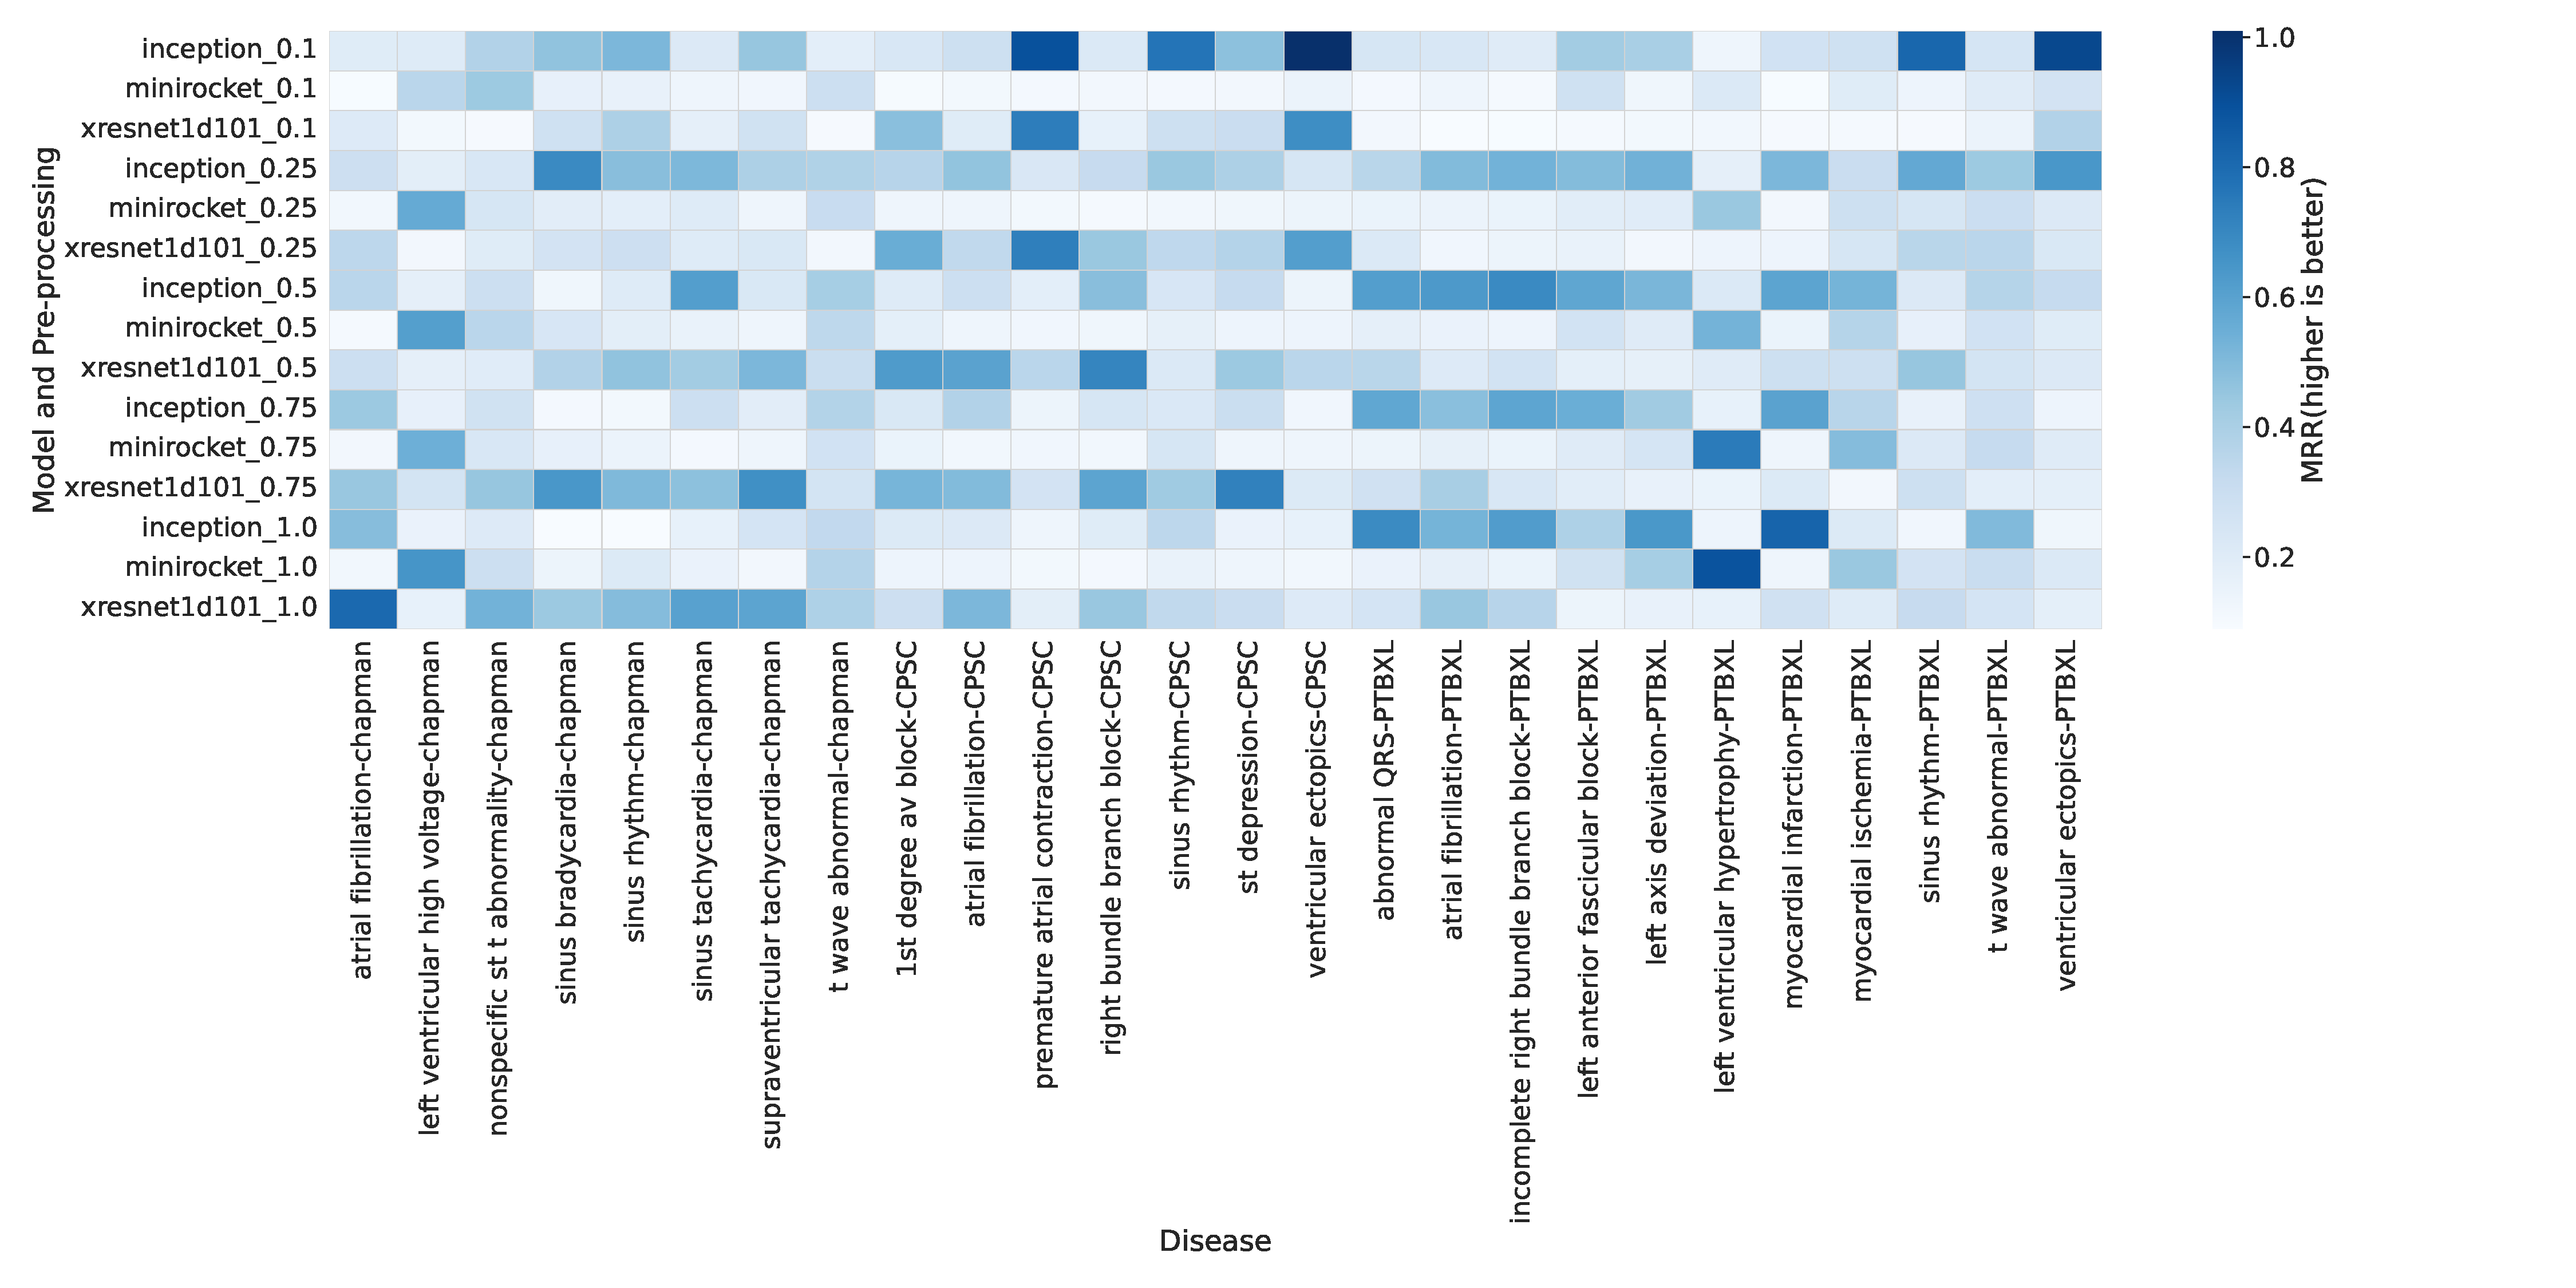
\includegraphics{images/Per-Disease_Model_Performance_all.pdf}}
  
  }
\end{figure*}
\section{Experiment Methodology}
\label{sec:experiment}

In Section~\ref{sec:prevwork} we discussed common pre-processing functions, and how some SOTA classifiers have used one or more of these functions, while others have omitted them entirely as seen in Table~\ref{tab:top5} as well as works by~\cite{ribeiro2020automatic}{\color{red}(should put in more works here)}. We also discussed three SOTA architectures for time-series classification, and in Section~\ref{datasets}, we described the three datasets of multi-labeled ECGs that the models can learn from. ~\textit{Best practices for ECG pre-processing can be established if we see consistent patterns of improvement in performance scores when applying a pre-processing function to different datasets, and comparing the performances of the models}. \\

To compare pre-processing methods, we apply the methods we want to compare to each dataset. For example, we would have the CPSC dataset at various sampling rates: CPSC\_500Hz, CPSC\_250Hz, etc. For each version of the dataset (i.e, the dataset pre-processed using a different function), we train and test each model 20 times. For 20 rounds, the data is randomly split in 80/10/10 training/validation/testing sets. Each model is trained on the training set, and the best model (according to the F1 score on the validation set) is saved to disk. When no improvements in the F1 measure is seen after 30 epochs, the training stops, and the best model's F1 score on the test set is saved as the performance score of the experiment. This means that for each dataset/pre-processing/model combination, we have 20 performance scores. 

In this case, we use the Wilcoxon signed rank test to measure whether each model out-performs every other model. To rank and compare the models, we use the Wilcox-Holm post-hoc analysis used for creating critical-difference diagrams by~\cite{IsmailFawaz2018deep}. This analysis shows whether the differences between each model pair is significant, and ranks each model. While~\cite{IsmailFawaz2018deep} uses the average rank to show relative performance, we use the "Mean Reciprocal Rank" (MRR) for each model. Here, $rank_i$ refers to the model's rank relative to the other models when trained/validated/tested on the same subsets of a dataset, and $Q=20$ since for each model/dataset combination we are "bootstrapping" 20 times:
\[ \text{MRR} = \frac{1}{Q}\sum_{i=1}^{Q}\frac{1}{rank_i} \]


\section{Scaling/Down-sampling}
\label{sec:scaling}
The scaling rates used here are 0.1, 0.25, 0.5, 0.75, and 1. When applied to the ECGs (all of which have the sampling rate of 500Hz), these scaling rates down-sample the signals to the corresponding sampling rates of 50Hz, 125Hz, 250Hz, 375Hz, and the unmodified 500Hz. Effectively, each dataset has 5 different sampling rates, and each of the 3 models learns from these datasets by randomly selecting 80\% of the dataset for training, 10\% for validation, and 10\% for testing. In total, for each dataset, we run 15 experiments (3 architectures, and 5 different sampling rates) and for each experiment, we measure 20 performance scores by running the training/validation/testing step and measuring the macro-average F1 score on the test set.~{\color{red} Show how high the performance cost for this is, in time and VRAM required}. We use the Wilcox-Holm post-hoc analysis described in the methodology (Section~\ref{sec:experiment}) to get the rank and relative performance for each model. 
\subsection{Downsampling Results}
These results are shown in Figure~\ref{fig:scaling_results_per_disease}. Here, no consistent pattern can be seen across diseases and scaling rates, however, some trends are observable. For example, for Atrial fibrillation which is common label in all 3 datasets, we see that DL models with higher sampling rates performed the best. Another interesting label is Sinus Rythm, also common in all 3 datasets,  where the inception network with lowest possible sampling rate clearly out-performs. {\color{red} which other patterns do we highlight?}\\

 {\color{red} Abram feedback: Show correlation between sampling rate and performance, and sampling rate and rank}
Readers interested in comparisons of the 3 models under different scaling conditions can see Appendix~\ref{apd:model_vs_model}. 

\section{Band-Pass Filtering}
\label{sec:BandPass}
A band-pass filter removes all frequencies outside its range, which can be an effective noise removal technique. The band-pass filter range applied to ECG data varies greatly in past works. Typically, the high-pass filter takes on a value of 0.05-1Hz, and the low-pass filter is applied somewhere between 30-150Hz~\cite{uwaechia2021comprehensive,luo2010review}.~{\color{red}there are a lot more works to cite here}. Is there an ``optimal" range for a band-pass filter in this context? Is band-pass filtering even necessary when using large datasets and large DL models?

In order to speed up training, we down-sample each dataset to 250Hz. We then apply 3 different band-pass filters to the data before training the 3 models. The 3 ranges are 1-30Hz, 1-50Hz, 1-100Hz. We also compare to the case when no filtering was applied to the dataset. 


\begin{table}[hbtp]
\floatconts
  {tab:example-booktabs}
  {\caption{A Table With Horizontal Lines}}
  {\begin{tabular}{|llll|l|}
  \toprule
  - & \bfseries CPSC & \bfseries Chap & \bfseries PTBX. & \bfseries All\\
  \midrule
  
  Incep.  & -0.154  & -0.036 & -0.003 & -0.055      \\
  Mini. & 0.017   & 0.010   & 0.0528   & 0.026       \\
  xres.    & -0.0925 & 0.0833  & 0.111    & 0.0536       \\
  \hline
  All & 0.148   & -0.070  & -0.217   & 0.0393      \\
  \bottomrule
  \end{tabular}}
\end{table}

\begin{table}[htbp]
\floatconts
  {tab:example-hline}
  {\caption{A Table With Horizontal and Vertical Lines}}%
  {%
    \begin{tabular}{|lllll|}
    \hline
    \abovestrut{2.2ex}\bfseries Dataset & \bfseries Result\\\hline
    \abovestrut{2.2ex}
          & CPSC    & Chap. & PTBX    & All  \\
          Incep.  & -0.154  & -0.036 & -0.003 & -0.055      \\
    % \belowstrut{0.2ex}Data4 & 0.09876\\\hline
    \end{tabular}
  }
\end{table}


% \begin{table}[]
% \begin{tabular}{lllll}
%           & CPSC    & Chap. & PTBX    & All  \\
% Incep.  & -0.154  & -0.036 & -0.003 & -0.055      \\
% Mini. & 0.017   & 0.010   & 0.0528   & 0.026       \\
% xres.    & -0.0925 & 0.0833  & 0.111    & 0.0536       \\
% All & 0.148   & -0.070  & -0.217   & 0.0393      
% \end{tabular}
% \caption{}
% \label{tab:sr_correlations}
% \end{table}

\section{Normalization}
\label{sec:Norm}


\bibliography{pmlr-sample}

\appendix
\section{First Appendix}\label{apd:model_vs_model}
\begin{figure*}[tbp]
 % Caption and label go in the first argument and the figure contents
 % go in the second argument
\floatconts
  {fig:image}
  {\caption{Model performance comparison for all datasets. Best models (those with the lowest average ranking) are higher on the y-axis.}}
  {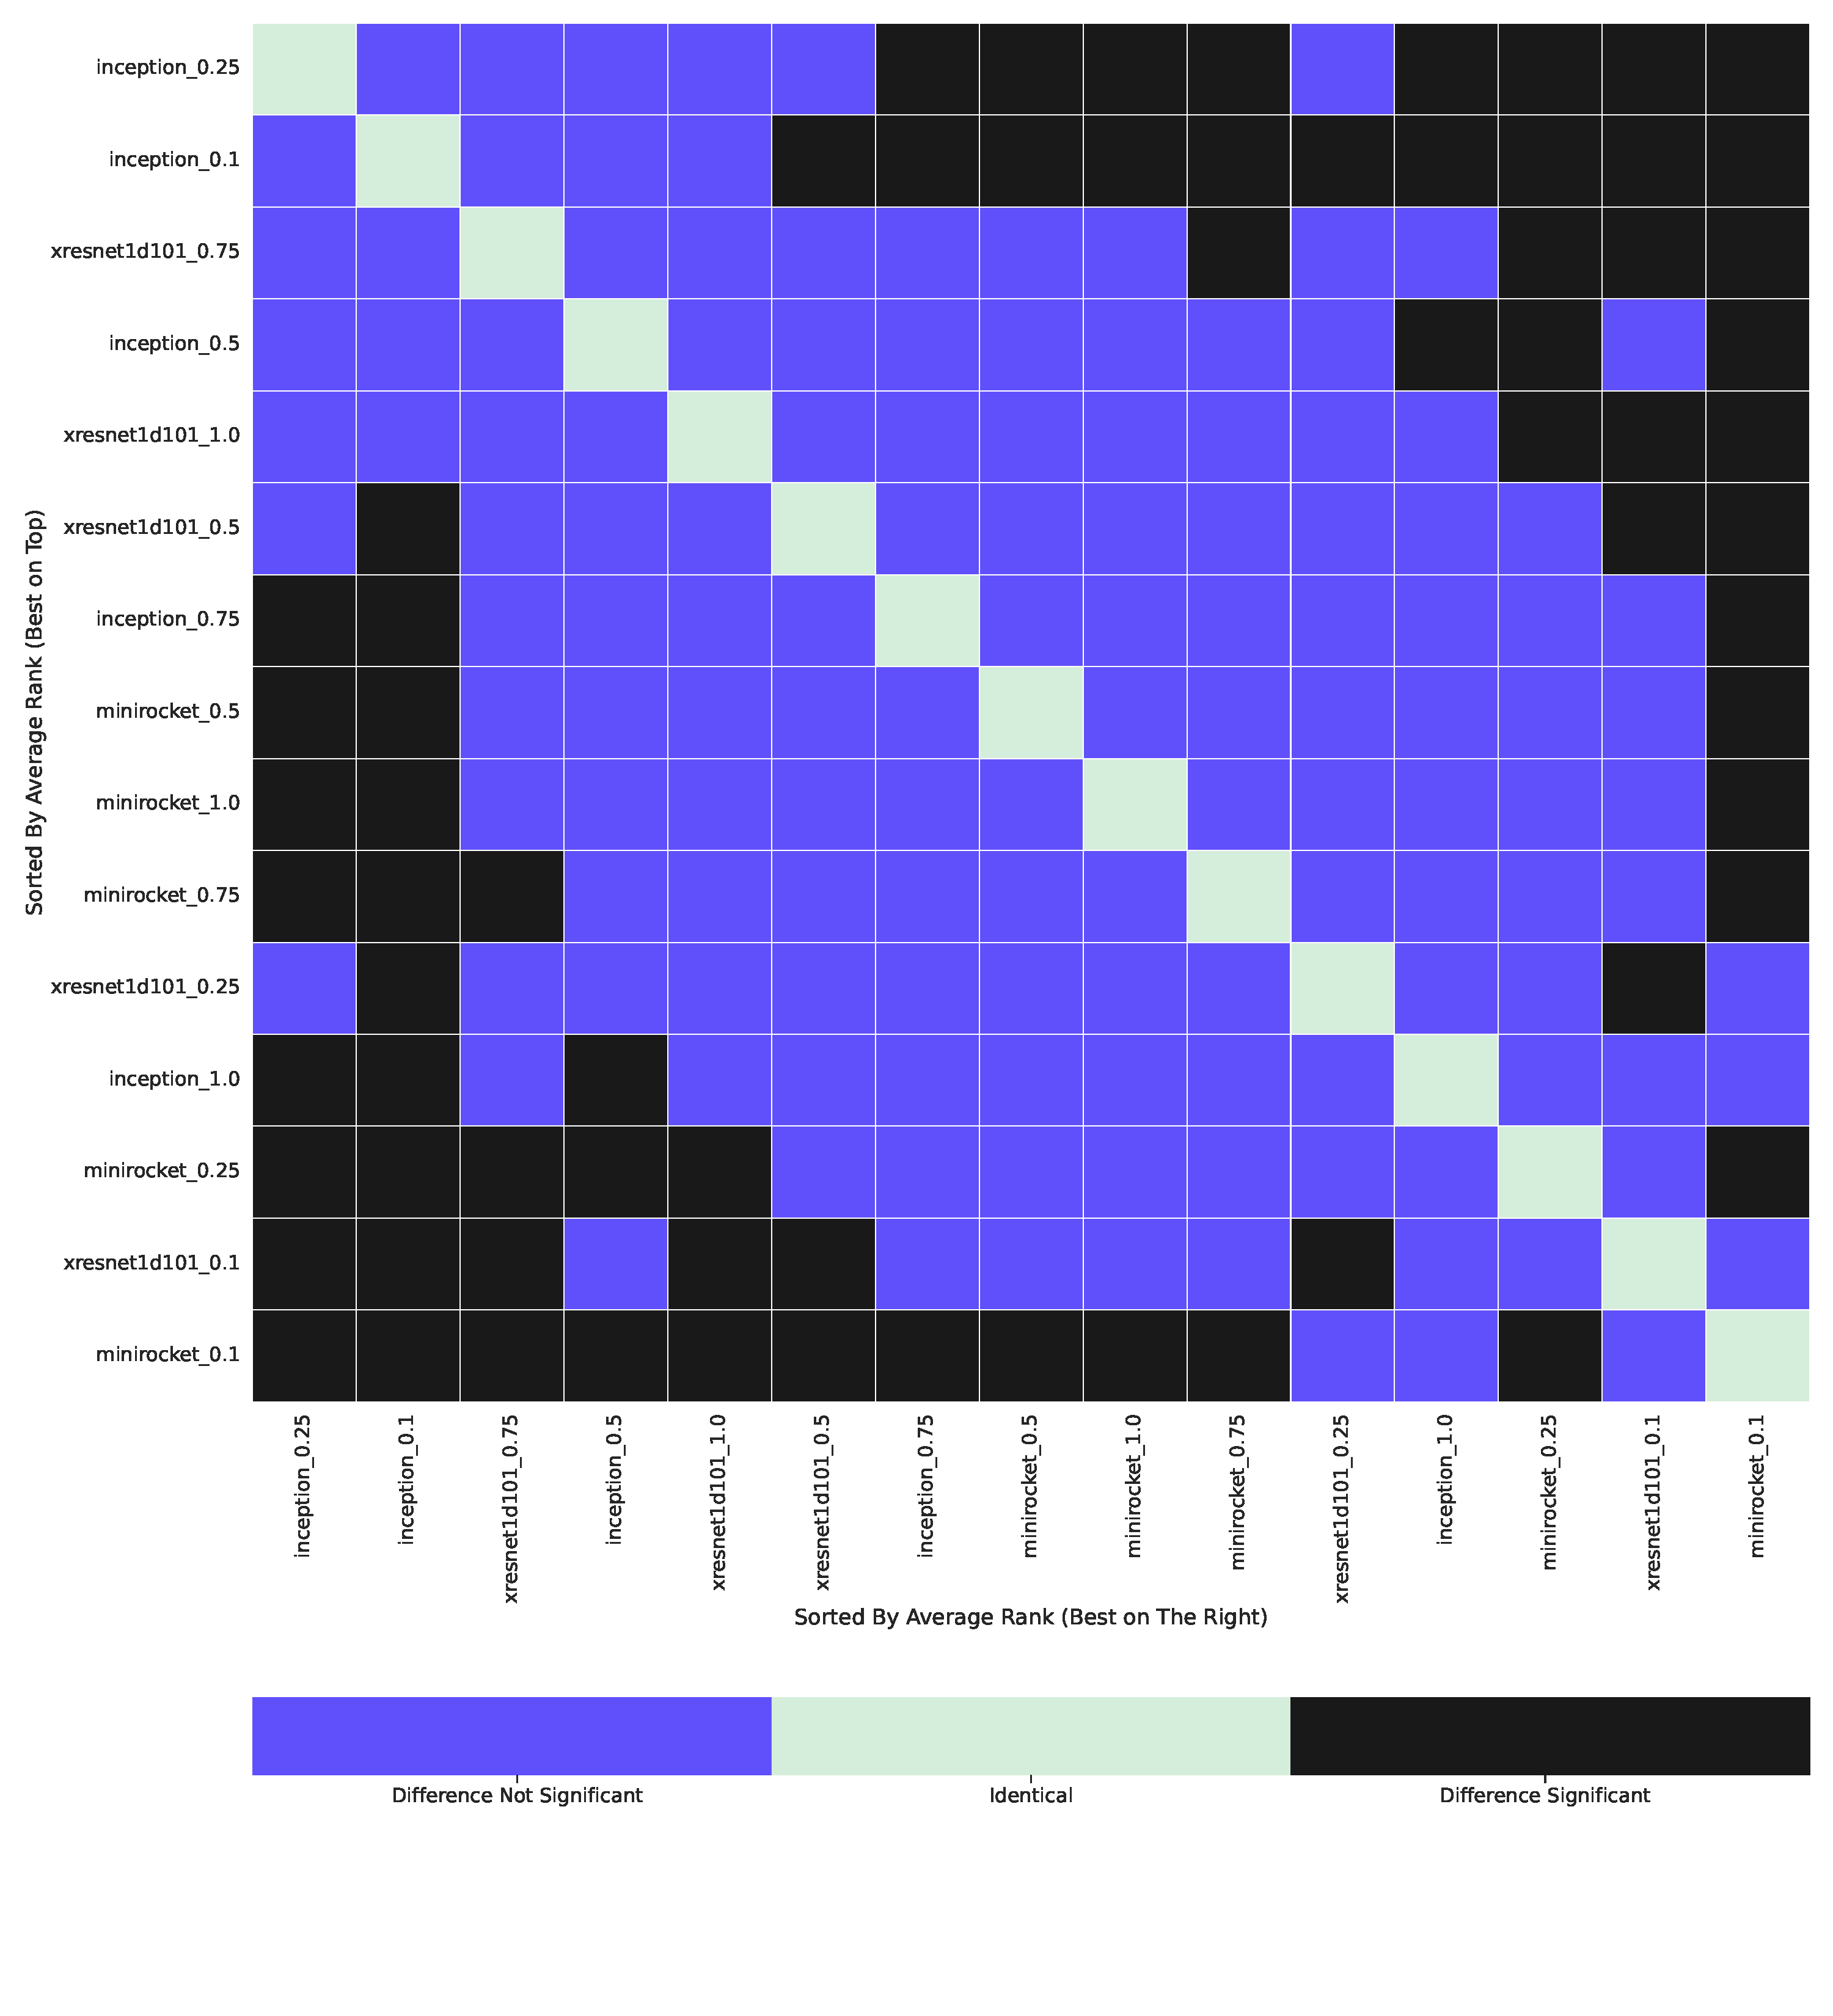
\includegraphics[width=1\linewidth]{images/model_comparisons_alldatasets.pdf}}
 
\end{figure*}

\begin{figure*}[tbp]
 % Caption and label go in the first argument and the figure contents
 % go in the second argument
\floatconts
  {fig:image}
  {\caption{Model performance comparison for CPSC}}
  {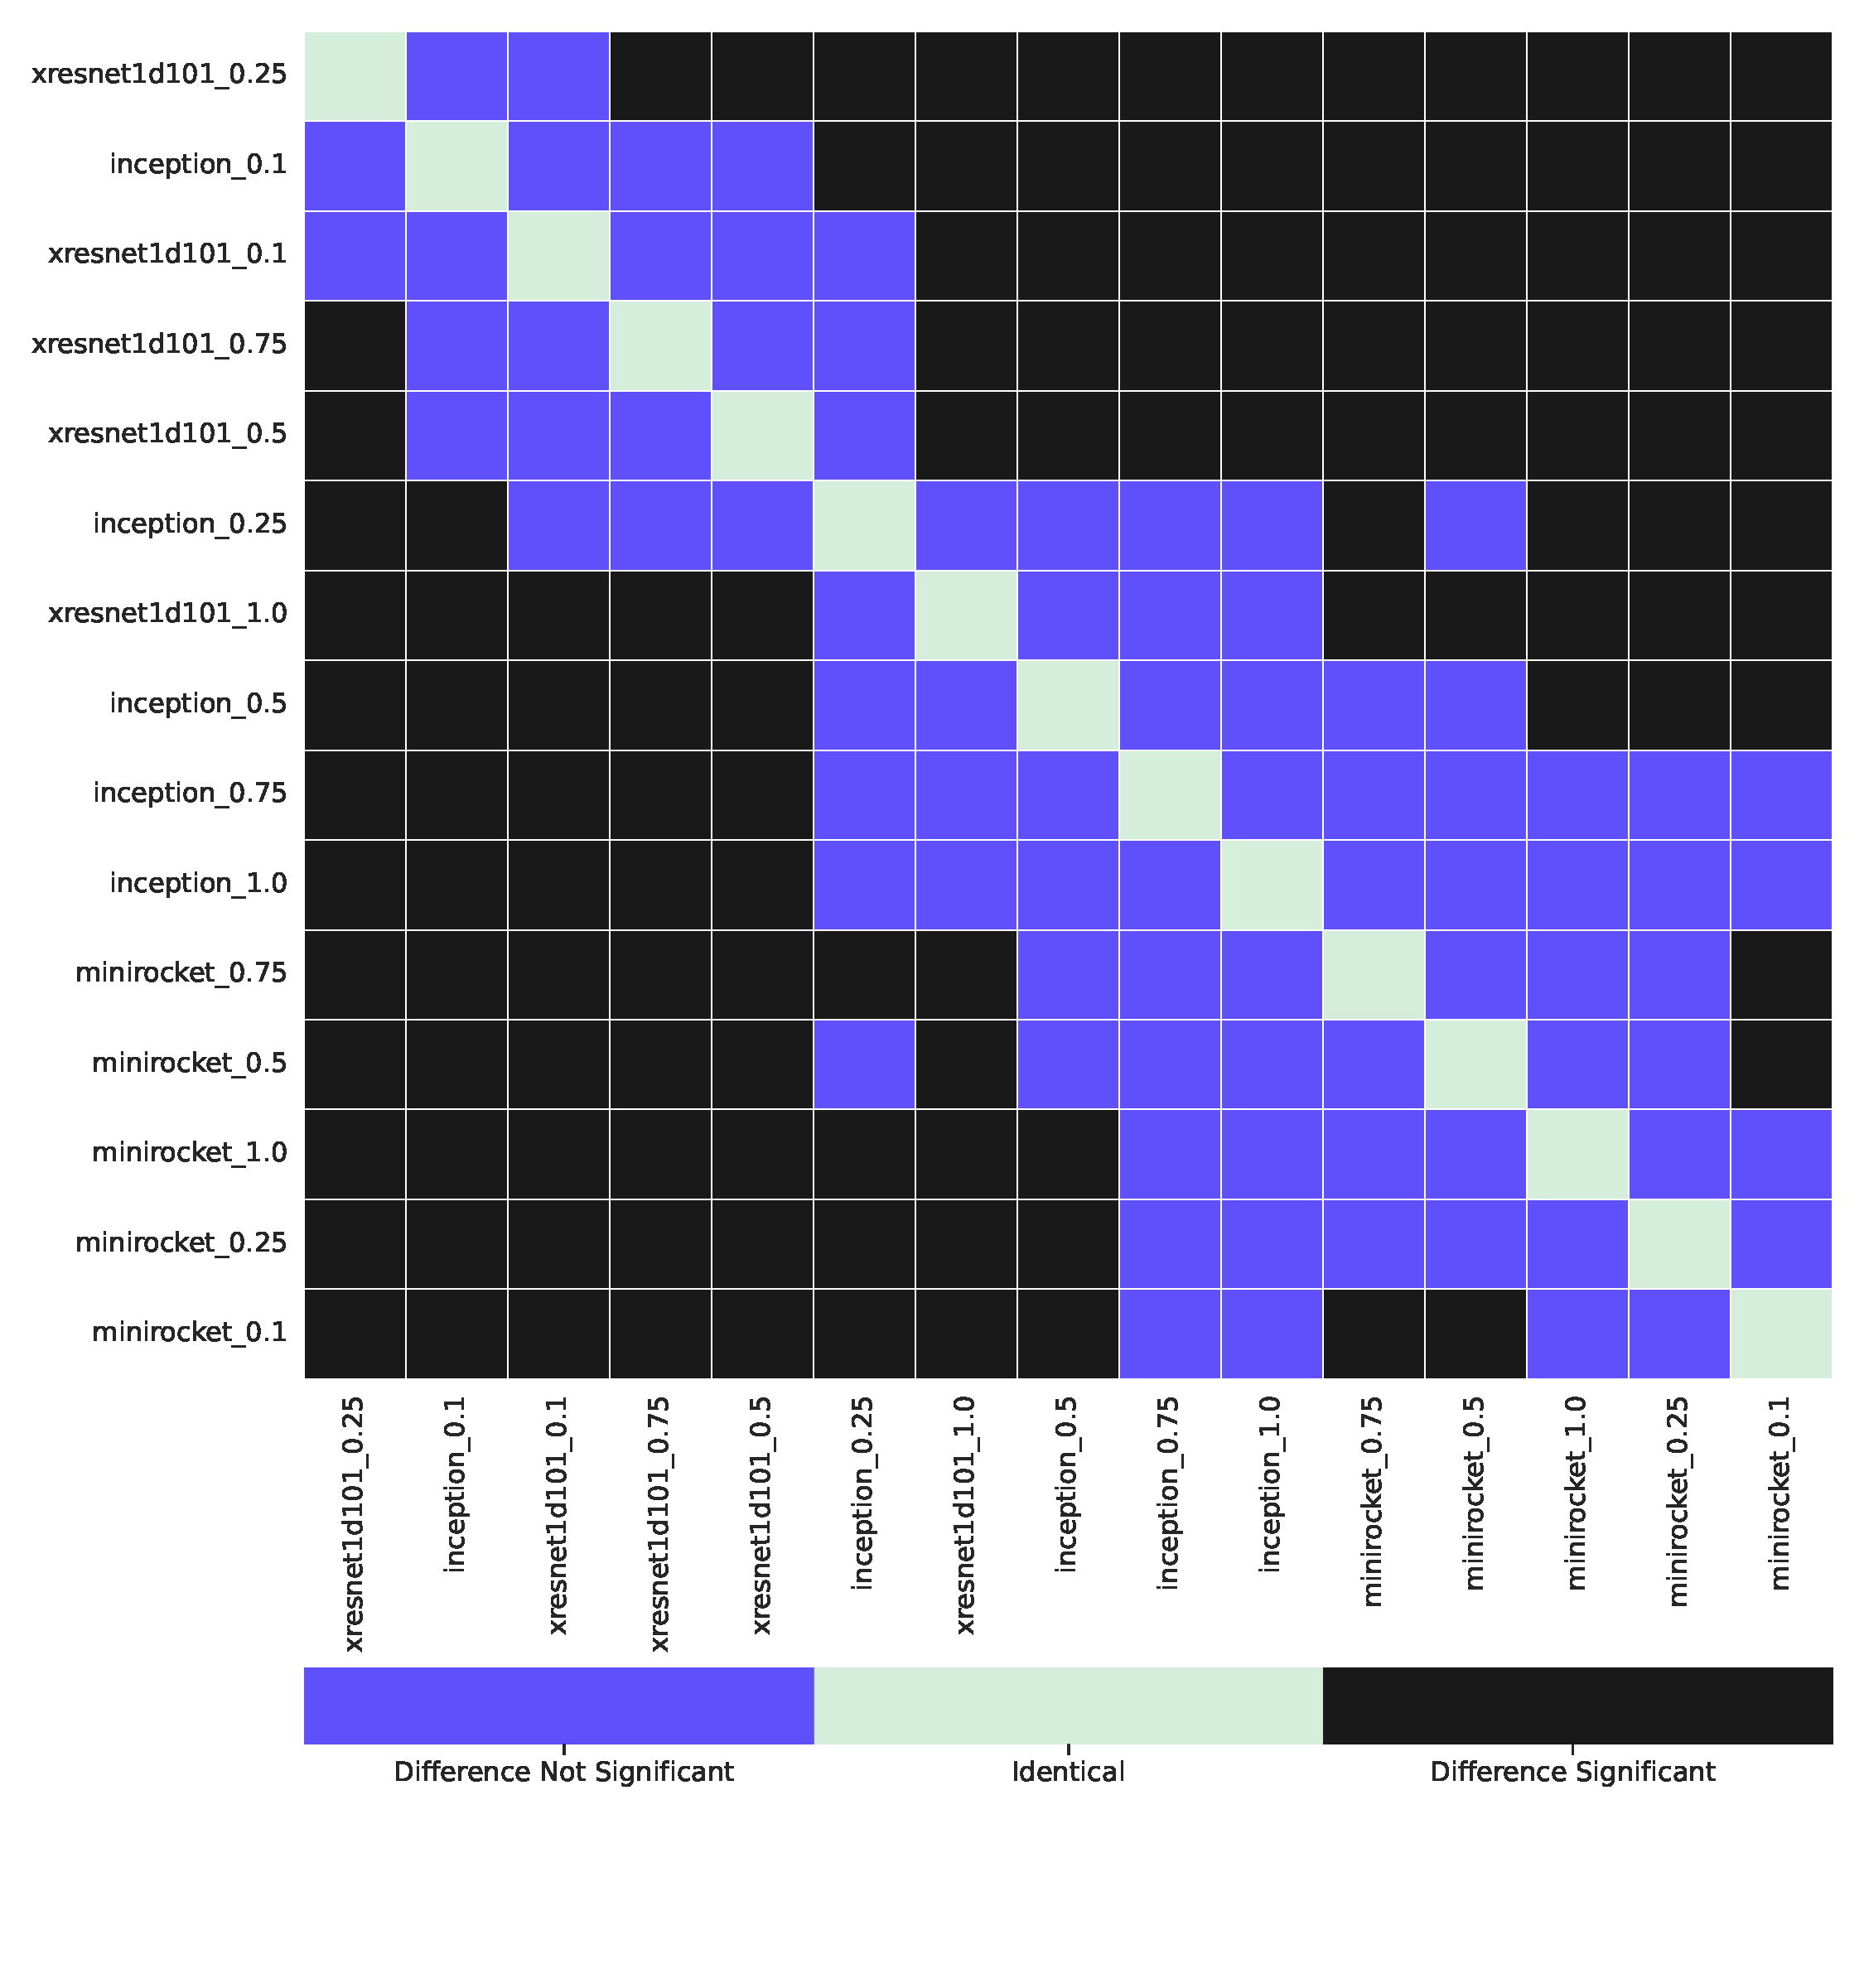
\includegraphics[width=1\linewidth]{images/model_comparisons_CPSC2018.pdf}}
 
\end{figure*}

\begin{figure*}[tbp]
 % Caption and label go in the first argument and the figure contents
 % go in the second argument
\floatconts
  {fig:image}
  {\caption{Model performance comparison for Chapman}}
  {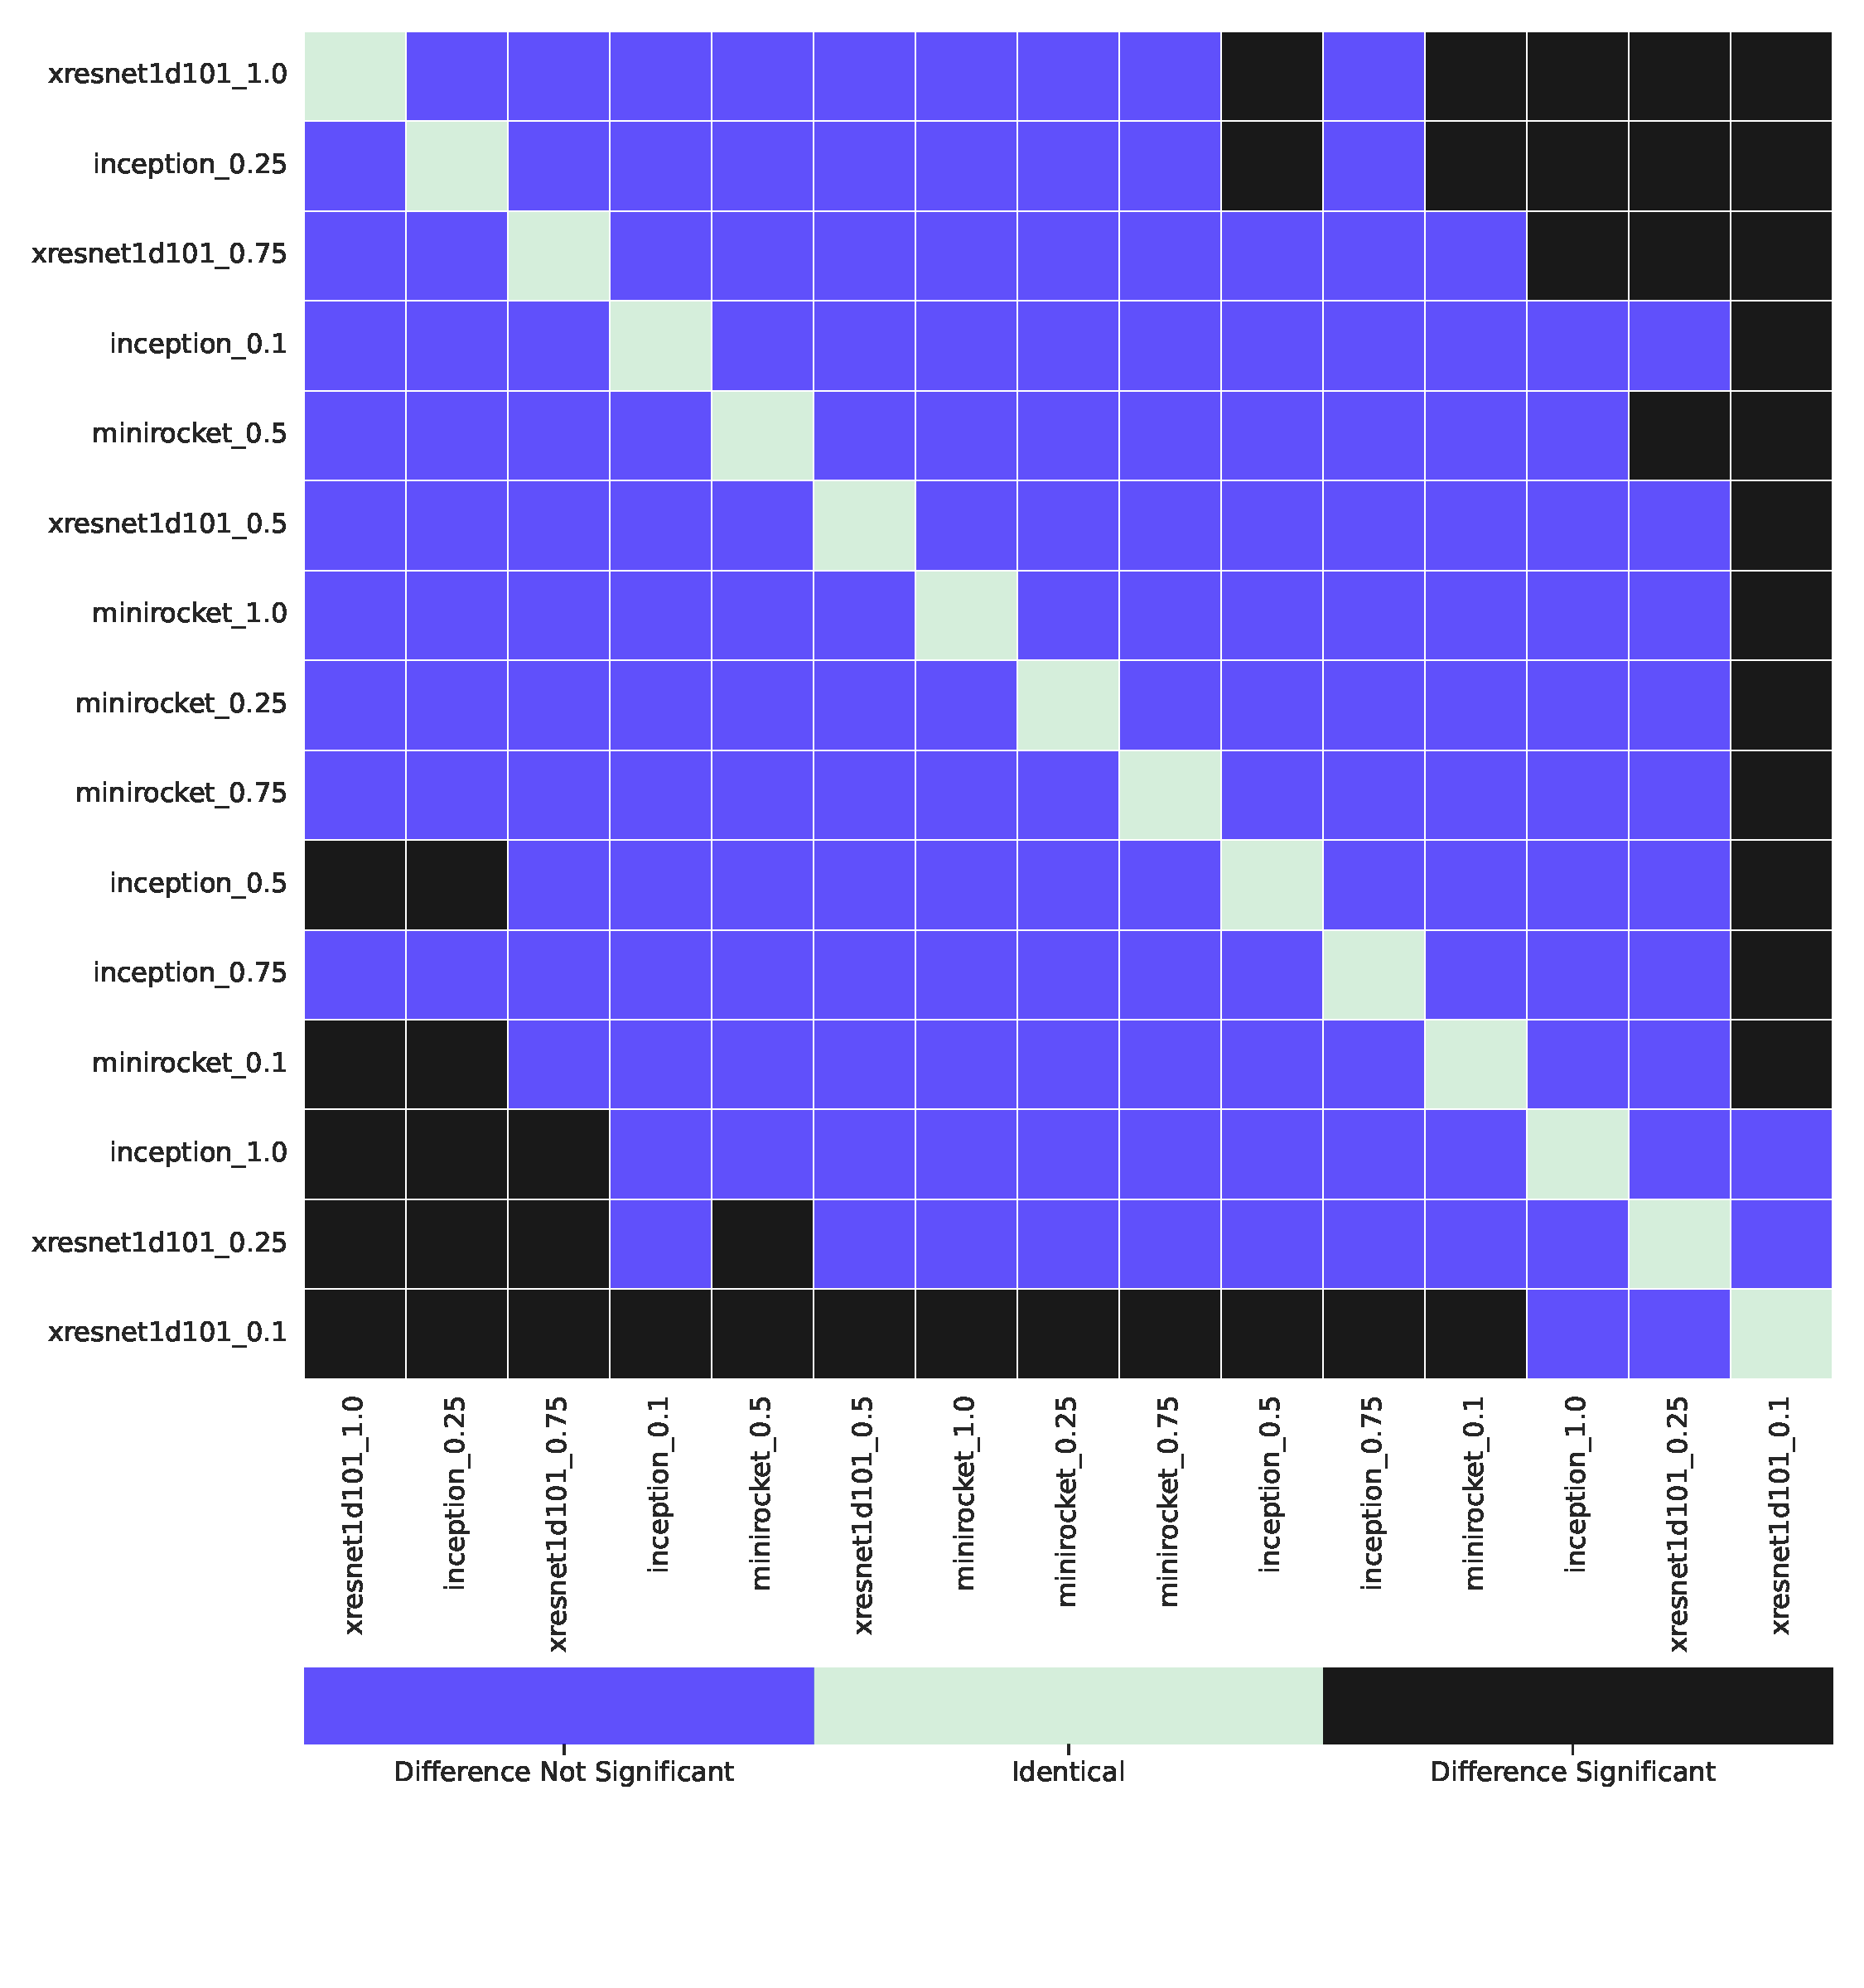
\includegraphics[width=1\linewidth]{images/model_comparisons_ChapmanShaoxing.pdf}}
 
\end{figure*}

\begin{figure*}[tbp]
 % Caption and label go in the first argument and the figure contents
 % go in the second argument
\floatconts
  {fig:image}
  {\caption{Model performance comparison for PTBXL}}
  {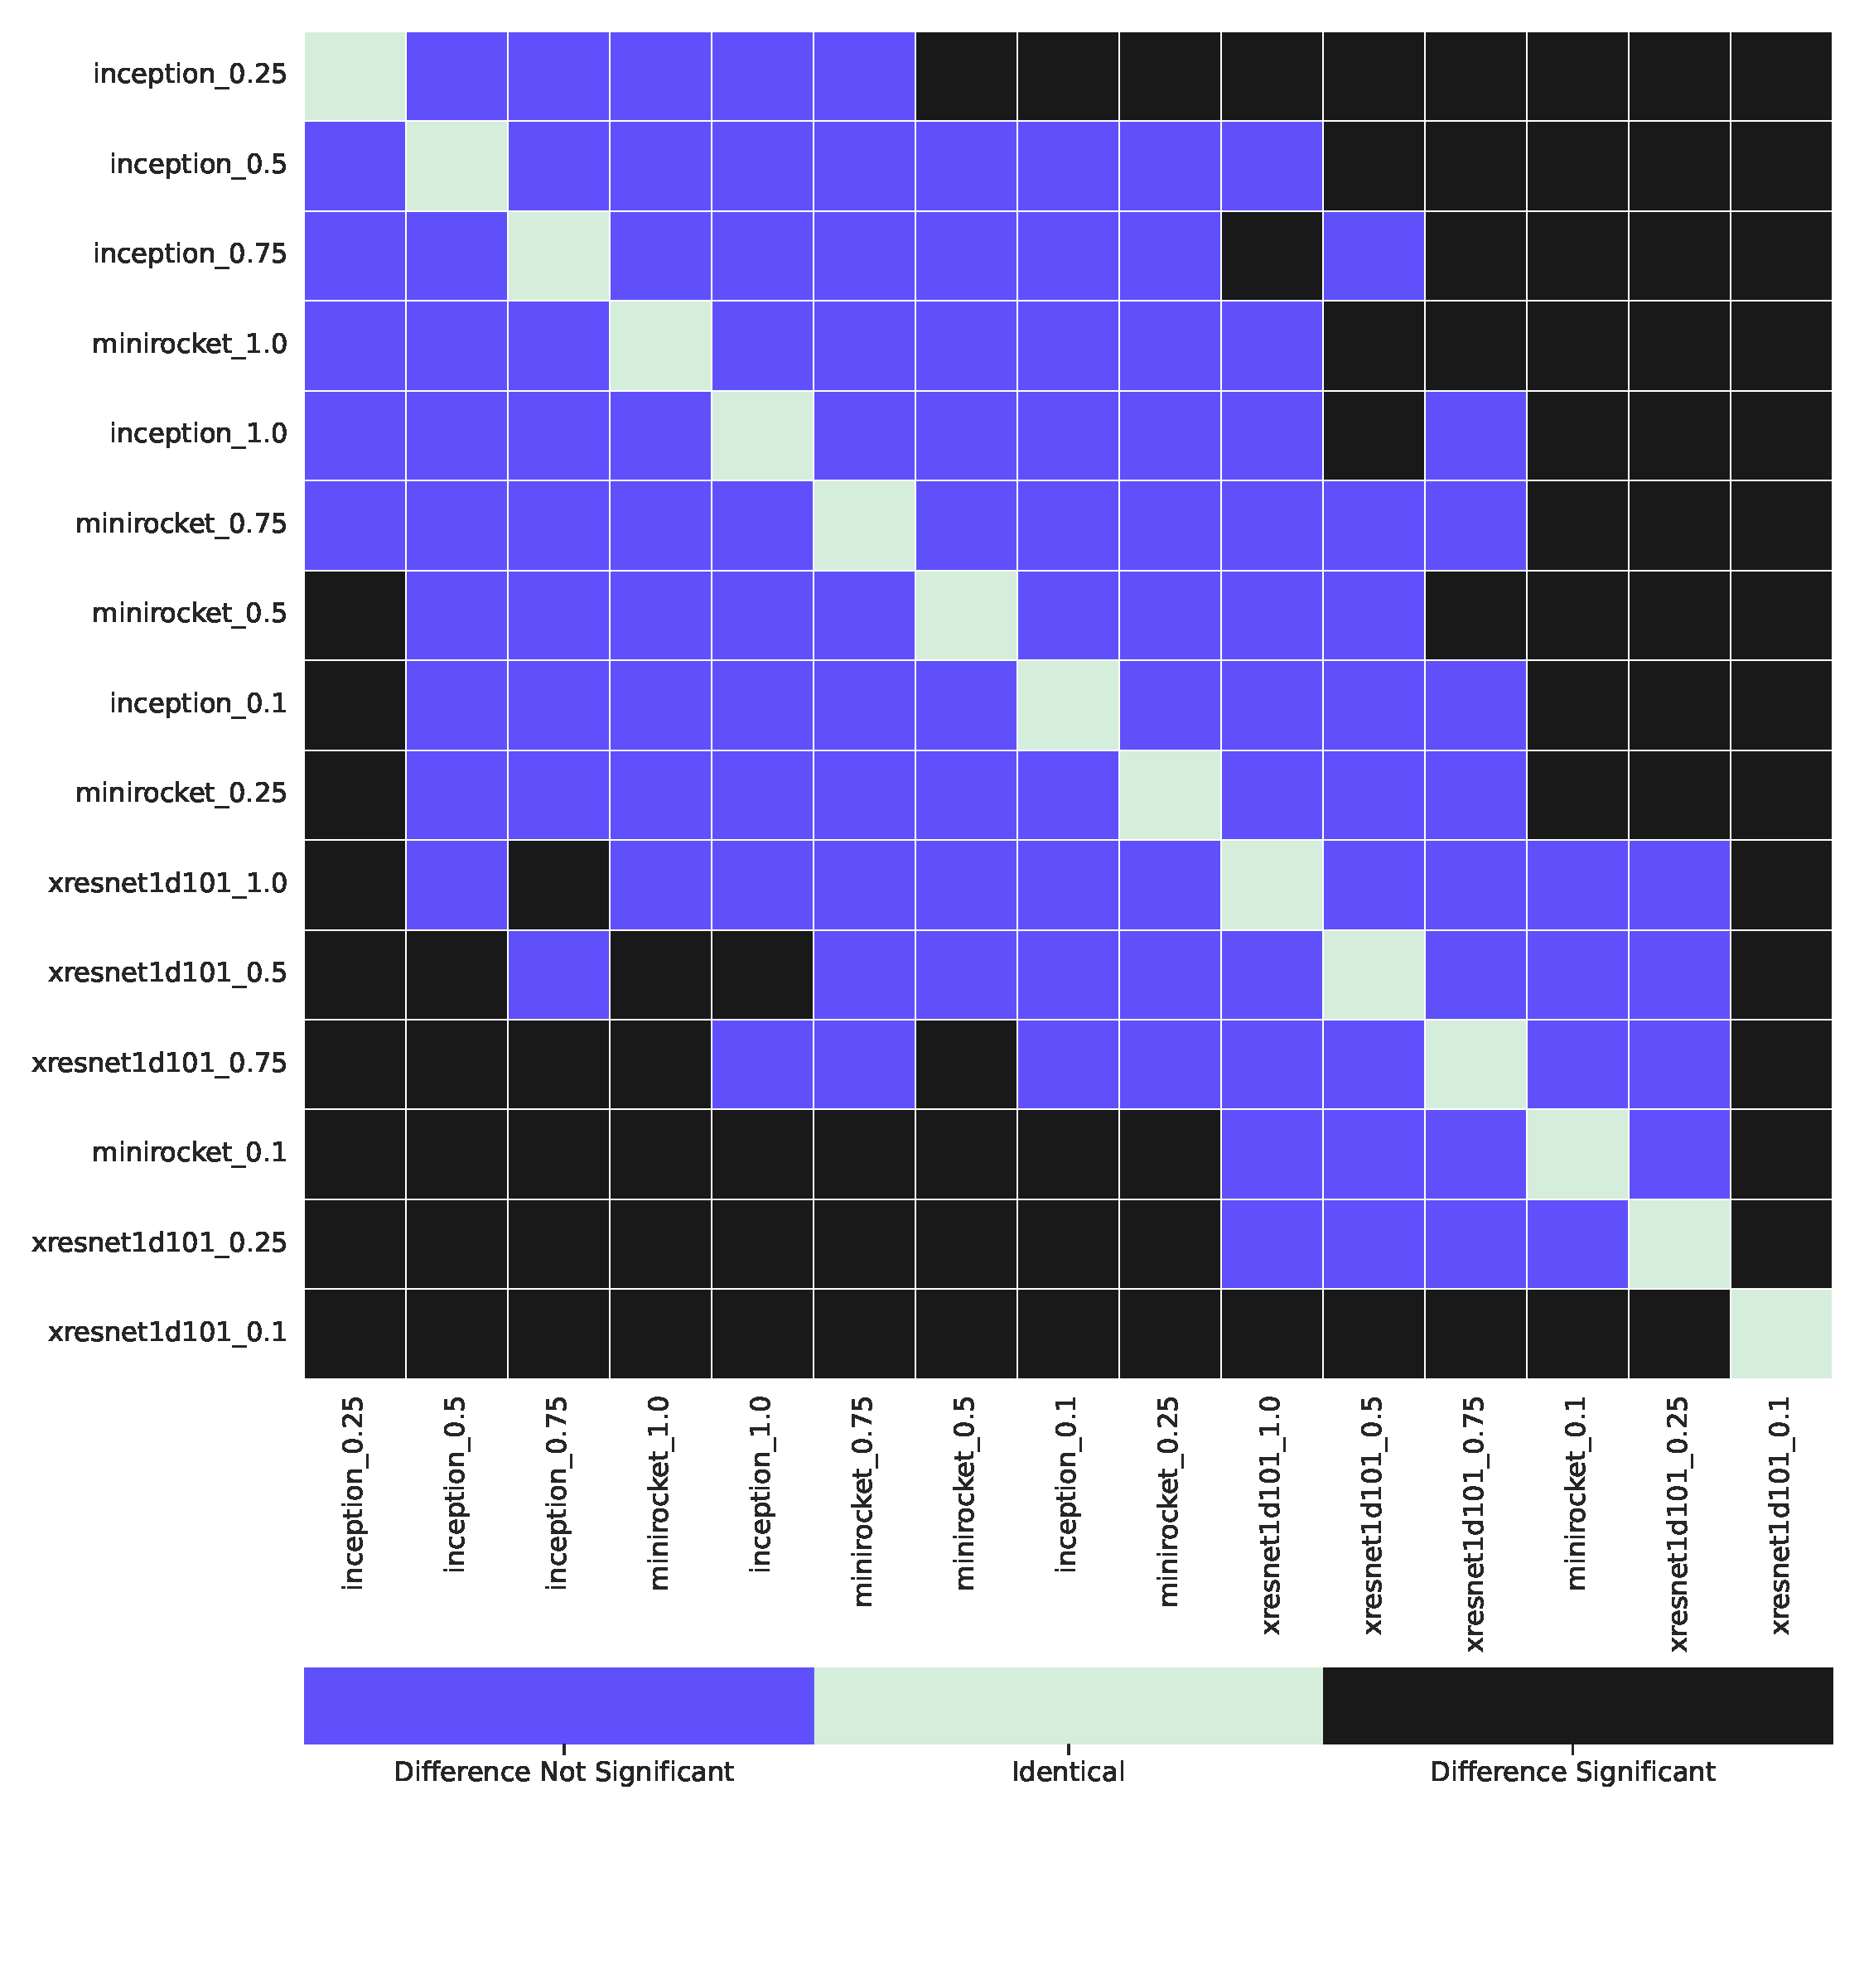
\includegraphics[width=1\linewidth]{images/model_comparisons_PTBXL.pdf}}
 
\end{figure*}

\end{document}
